%%% Relatorio Tecnico - Suficiencia Sistemas Embarcados - UTFPR
\documentclass[12pt,a4paper,brazil]{article}
\newcommand{\workingDate}{8 de outubro de 2026}
\newcommand{\userName}{Embarcados}
\newcommand{\institution}{UTFPR-AP}
% Evita conflito com xcolor carregado primeiro pelo TikZ dentro do estilo original.
\PassOptionsToPackage{usenames,dvipsnames}{xcolor}
\usepackage{researchdiary_png}
\usepackage{listings}
\usepackage{float}
\usepackage{placeins}
\usepackage{booktabs}
\usepackage{longtable}
\usepackage{tabularx}
\newcolumntype{Y}{>{\raggedright\arraybackslash}X}
\usepackage{graphicx}
\usepackage{array}
\usepackage{xcolor}
\usepackage{tikz}
\usepackage{pgfplots}
\usetikzlibrary{arrows.meta,positioning}
\pgfplotsset{compat=1.18}
\graphicspath{{figuras/}}
\hypersetup{hidelinks,pdftitle={Alarme e Relogio com FreeRTOS},pdfauthor={Pedro Lucas dos Reis Silva}}
\setlength{\emergencystretch}{2em}
\newcolumntype{P}[1]{>{\raggedright\arraybackslash}p{#1}}
\lstdefinestyle{cpp}{
    language=C++,
    basicstyle=\ttfamily\footnotesize,
    keywordstyle=\color{blue}\bfseries,
    commentstyle=\color{gray}\itshape,
    stringstyle=\color{red},
    numbers=left,
    numberstyle=\tiny\color{gray},
    numbersep=5pt,
    frame=single,
    breaklines=true,
    captionpos=b,
    tabsize=2,
    inputencoding=utf8,
    extendedchars=true,
    literate=
        {á}{{\'a}}1 {à}{{\`a}}1 {â}{{\^a}}1 {ã}{{\~a}}1
        {é}{{\'e}}1 {ê}{{\^e}}1
        {í}{{\'i}}1
        {ó}{{\'o}}1 {ô}{{\^o}}1 {õ}{{\~o}}1
        {ú}{{\'u}}1
        {ç}{{\c{c}}}1
        {Á}{{\'A}}1 {À}{{\`A}}1 {Â}{{\^A}}1 {Ã}{{\~A}}1
        {É}{{\'E}}1 {Ê}{{\^E}}1
        {Í}{{\'I}}1
        {Ó}{{\'O}}1 {Ô}{{\^O}}1 {Õ}{{\~O}}1
        {Ú}{{\'U}}1
        {Ç}{{\c{C}}}1
}




\begin{document}
\begin{center}
{\textbf{\LARGE Relógio e alarme com FreeRTOS}}\\[3mm]
{\large Exame de Suficiência --- Sistemas Embarcados 2026.2}\\[3mm]
Pedro Lucas dos Reis Silva --- RA 2272040\\
Engenharia de Computação --- UTFPR Apucarana\\
Professor Adalberto Lazarini\\[2mm]
8 de outubro de 2026
\end{center}
\section{Introdução}

O presente relatório descreve o desenvolvimento de um relógio e alarme para o exame de suficiência de Sistemas Embarcados. O enunciado solicita o uso de Arduino e RTOS, exibição local de data e hora, ajuste por botão ou joystick, configuração de alarme e função soneca. O protótipo utiliza Arduino Mega 2560, LCD 1602A, joystick, botão, buzzer e LED. A operação ocorre pela interface física; o computador fornece alimentação e, durante o ajuste inicial, uma referência visual de horário. \autocite{fonte1}

A solução separa aquisição de entrada, controle do relógio, sinalização e apresentação. Cada tarefa possui uma responsabilidade, e a comunicação ocorre por eventos e cópias de estado em filas. O Timer1 fornece a contagem usada pelo calendário e pelos prazos de alarme; o watchdog mantém o tick do escalonador. Essa separação permite atualizar o LCD e navegar no menu enquanto o relógio continua avançando.

\section{Protótipo e interface}

O LCD opera em modo paralelo de quatro bits. O potenciômetro ajusta exclusivamente o contraste no terminal V0: não há controle de volume no programa. O botão D5 e o clique do joystick utilizam \texttt{INPUT\_PULLUP}, com acionamento em nível baixo. No Mega, \texttt{A0} e \texttt{A1} são constantes numéricas equivalentes a 54 e 55. A implementação conserva essa pinagem. A configuração fica em SRAM; após reinicialização, vale o estado inicial definido no sketch.

\begin{center}\small
\begin{tabularx}{\textwidth}{@{}YYY@{}}\toprule

\textbf{Componente} & \textbf{Conexão no Mega} & \textbf{Função} \\ \midrule

LCD RS / E & 22 / 23 & Seleção e habilitação \\

LCD D4 / D5 / D6 / D7 & 24 / 25 / 26 / 27 & Dados em quatro bits \\

Joystick X / Y / SEL & 54 (A0) / 55 (A1) / 2 & Navegação e seleção \\

Botão de soneca & 5, botão ao GND & Ação dependente do estado \\

Buzzer / LED & 8 / 9 & Aviso sonoro e visual \\

Potenciômetro de contraste & Cursor ao V0; extremos a 5 V e GND & Legibilidade do LCD \\

\bottomrule\end{tabularx}
\end{center}

O clique curto em SEL abre o menu e, ao final, salva o conjunto editado. O movimento horizontal seleciona hora, minuto, segundo, dia, mês, ano, hora do alarme, minuto do alarme ou soneca; o movimento vertical altera o valor. O cursor identifica o campo. O programa mantém um rascunho separado e aplica a edição ao salvar. Assim, alterar apenas o alarme não restaura um horário antigo nem interrompe a contagem corrente.

\begin{center}\small
\begin{tabularx}{\textwidth}{@{}YYY@{}}\toprule

\textbf{Situação} & \textbf{Ação física} & \textbf{Resultado} \\ \midrule

Tela normal & Clique SEL & Abre a edição \\

Edição & Esquerda/direita; cima/baixo & Seleciona campo; altera valor \\

Edição & Clique SEL / D5 & Salva / cancela o rascunho \\

Tela normal & D5 & Habilita ou desabilita o alarme \\

Alarme tocando & D5 ou clique SEL & Inicia a mesma soneca configurada \\

Soneca em curso & D5 & Cancela a soneca e desabilita o alarme \\

Qualquer estado & SEL mantido por 1 s & Encerra o aviso e cancela a edição \\

\bottomrule\end{tabularx}
\end{center}

A soneca admite de 1 a 10 minutos, com valor inicial de 5 minutos. Cada toque dura até 60 segundos. A repetição da soneca depende de novo acionamento enquanto o alarme toca; não existe repetição automática ilimitada. O encerramento por SEL longo mantém a habilitação diária, enquanto D5 durante a soneca também a desabilita.

\begin{figure}[htbp]
\centering
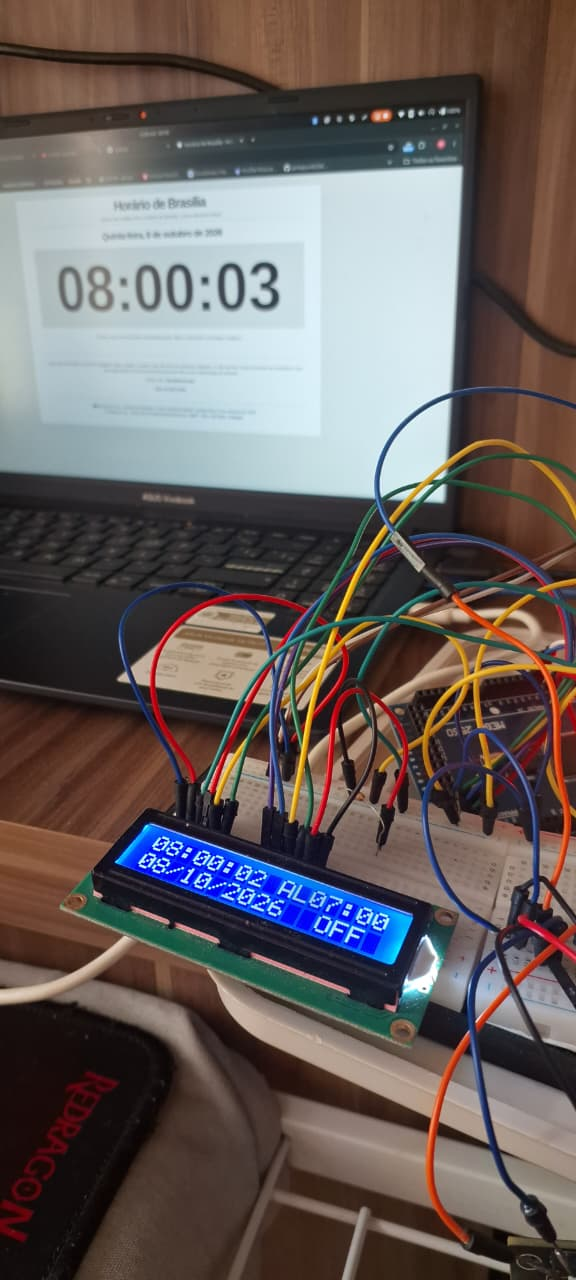
\includegraphics[height=8.1cm]{figuras/01_relogio_referencia.jpg}\hspace{3mm}
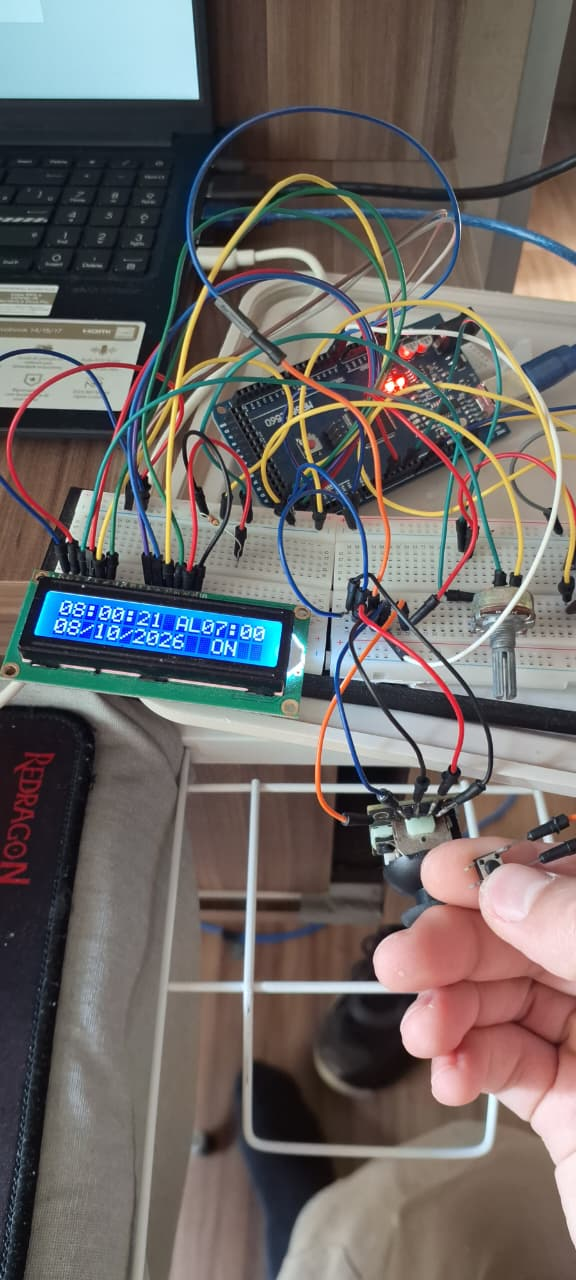
\includegraphics[height=8.1cm]{figuras/02_alarme_habilitado.jpg}\hspace{3mm}
\caption{Protótipo em operação: alinhamento inicial com referência visual e indicação de alarme habilitado. Fonte: registro do autor, 08/10/2026.}\label{fig:operacao}
\end{figure}

\section{FreeRTOS, bare metal e máquina de estados}

Em uma implementação bare metal com laço principal, a aplicação determina diretamente a ordem de leitura, cálculo e exibição. Uma chamada demorada pode retardar a próxima leitura, caso o projeto concentre toda a execução no mesmo fluxo. Uma máquina de estados cooperativa, associada a interrupções e temporização sem espera ocupada, também pode executar corretamente este relógio, com menor consumo de memória e menor custo de troca de contexto.

O FreeRTOS acrescenta escalonamento preemptivo, prioridades, filas e estados de execução para cada tarefa. No ATmega2560, existe apenas um núcleo: a concorrência resulta da alternância de contexto, não da execução simultânea de quatro tarefas. Quando a tarefa de alarme fica pronta, sua prioridade permite preemptar a atualização do display. Quando uma tarefa aguarda uma fila ou um prazo do kernel, ela fica bloqueada e libera a CPU.

Máquina de estados e RTOS não são alternativas excludentes. A solução utiliza o RTOS para organizar a concorrência e uma máquina de estados dentro da tarefa de relógio para representar silêncio, toque, soneca e edição. O benefício é separar a política da aplicação da execução dos periféricos. A configuração preemptiva também habilita divisão de tempo entre tarefas prontas de mesma prioridade: relógio e botões compartilham o nível 2. A prioridade define a escolha entre tarefas prontas, não uma reserva fixa de tempo de CPU. O custo adicional envolve pilha por tarefa, memória de filas, troca de contexto e cuidado com sincronização. Portanto, o uso do RTOS atende ao objetivo didático e torna explícita a coordenação de atividades concorrentes; ele não transforma o oscilador em uma referência de horário mais precisa.

\section{Arquitetura por eventos e diferença entre fila e mutex}

A tarefa de relógio possui a única instância autoritativa de \texttt{Estado}. A tarefa de botões envia valores do tipo \texttt{Evento}; a tarefa de relógio processa cada evento, atualiza o estado e publica a saída. A tarefa de display recebe uma cópia consistente, denominada snapshot. A tarefa de alarme recebe somente a condição desejada de acionamento.

\begin{figure}[htbp]
\centering
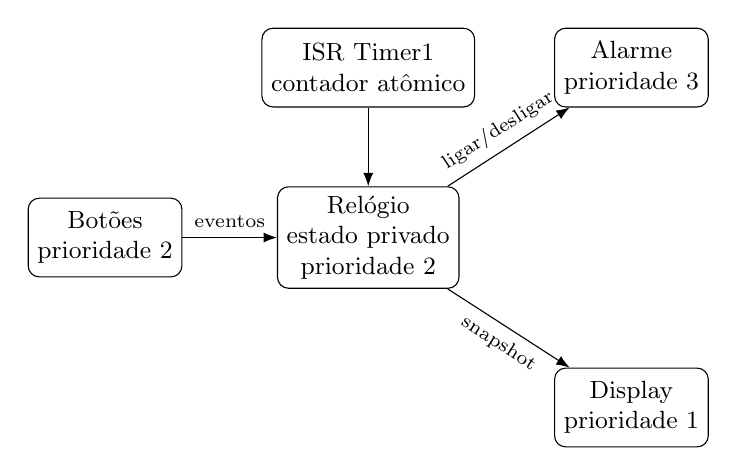
\begin{tikzpicture}[node distance=10mm and 12mm,box/.style={draw,rounded corners,align=center,minimum height=10mm,font=\small},>=Latex]
\node[box] (b) {Botões\\prioridade 2};
\node[box,right=of b] (r) {Relógio\\estado privado\\prioridade 2};
\node[box,above right=of r] (a) {Alarme\\prioridade 3};
\node[box,below right=of r] (d) {Display\\prioridade 1};
\node[box,above=of r] (t) {ISR Timer1\\contador atômico};
\draw[->] (b) -- node[above,font=\scriptsize]{eventos} (r);
\draw[->] (t) -- (r);
\draw[->] (r) -- node[above,sloped,font=\scriptsize]{ligar/desligar} (a);
\draw[->] (r) -- node[below,sloped,font=\scriptsize]{snapshot} (d);
\end{tikzpicture}
\caption{Fluxo de comunicação e propriedade do estado. A ISR publica contagens; a tarefa de relógio interpreta o tempo e a entrada.}
\end{figure}

\begin{center}\small
\begin{tabularx}{\textwidth}{@{}YYY@{}}\toprule

\textbf{Canal} & \textbf{Capacidade e conteúdo} & \textbf{Política} \\ \midrule

\texttt{entradas} & 16 eventos & FIFO; envio sem espera \\

\texttt{saidaTela} & 1 snapshot & Substitui a imagem antiga \\

\texttt{saidaAlarme} & 1 booleano & Conserva o último estado desejado \\

\bottomrule\end{tabularx}
\end{center}

A fila de entrada conserva a ordem dos comandos aceitos. Se estiver cheia, o produtor registra a perda por notificação contadora; a interface apresenta “REPITA O COMANDO”. O envio com tempo zero evita reter a tarefa de entrada, mas não significa capacidade infinita. O controle processa no máximo 16 eventos por passagem, evitando que um fluxo de entrada monopolize indefinidamente o ciclo.

A saída do display tem semântica diferente: importa apresentar o estado mais recente, sem reproduzir uma sequência de telas antigas. A caixa de uma posição permite \texttt{xQueueOverwrite}. A mesma política no alarme evita manter um comando de desligamento atrás de comandos desatualizados. O consumidor recebe o estado final vigente; a caixa não representa um histórico de cada transição intermediária.

Na versão com mutex, a tarefa obtém exclusividade para acessar uma estrutura compartilhada e depois devolve o recurso. O mutex não transporta dados e não organiza uma sequência de comandos. No FreeRTOS, o mutex oferece herança de prioridade: quando uma tarefa de alta prioridade espera por ele, o kernel pode elevar temporariamente a prioridade de quem o possui. Isso reduz o efeito da inversão de prioridade, mas não elimina o tempo necessário para liberar o recurso. \autocite{fonte2}

\begin{center}\small
\begin{tabularx}{\textwidth}{@{}YYY@{}}\toprule

\textbf{Aspecto} & \textbf{Estado compartilhado com mutex} & \textbf{Estado com dono único e filas} \\ \midrule

Acesso & Exige adquirir e liberar exclusividade & O controlador altera seu estado privado \\

Comunicação & Leitura/escrita do objeto comum & Cópia de evento ou snapshot \\

Prioridade & Pode exigir herança de prioridade & LCD não retém um lock necessário ao controle \\

Custo & Pouca cópia, disciplina de bloqueio & Buffer e cópia, política de capacidade \\

\bottomrule\end{tabularx}
\end{center}

A implementação final elimina a disputa por um mutex de aplicação entre display, relógio e alarme. Isso remove esse caminho de inversão de prioridade e evita acesso concorrente ao estado civil. A garantia decorre da propriedade do estado e da política de comunicação, não da mera existência de filas. O kernel ainda utiliza proteção interna breve, e a comunicação entre ISR e tarefa exige atomicidade própria.

\section{Base de tempo, registradores e tick}

\subsection{Papel de cada temporizador}

\begin{center}\small
\begin{tabularx}{\textwidth}{@{}YYY@{}}\toprule

\textbf{Recurso} & \textbf{Base utilizada} & \textbf{Responsabilidade no programa} \\ \midrule

Watchdog & Oscilador interno próprio & Tick do FreeRTOS \\

Timer0 & Clock principal dividido por 64 & \texttt{millis()} e \texttt{micros()} do core Arduino \\

Timer1 & Clock principal dividido por 64 & Contagem do relógio a 100 Hz \\

Timer2 & Configuração interna de \texttt{tone()} & Onda sonora do buzzer \\

\bottomrule\end{tabularx}
\end{center}

Timer0 não é um RTC de calendário neste projeto. O core utiliza seu overflow de 8 bits, nominalmente a cada 1,024 ms em 16 MHz, e compensa a fração para construir \texttt{millis()}. Essa função representa tempo desde a inicialização e aparece no diagnóstico; o calendário utiliza Timer1. Como Timer0 e Timer1 derivam do mesmo clock principal, a concordância entre ambos ajuda a verificar a implementação, mas não comprova exatidão perante uma referência externa. \autocite{fonte3}

O Timer2 fica reservado à implementação de \texttt{tone()} no core AVR utilizado. Não existe conflito direto com Timer1 nesta configuração. A troca de funções dos temporizadores exigiria revisar a biblioteca que utiliza cada periférico. \autocite{fonte4}

\subsection{Timer1 em CTC}

O modo CTC reinicia o contador quando ocorre a comparação com \texttt{OCR1A}. Com clock nominal de 16 MHz, prescaler 64 e \texttt{OCR1A = 2499}, a frequência de comparação é:

\[f_{comparacao}=\frac{16\,000\,000}{64(2499+1)}=100\;\mathrm{Hz},\qquad T=10\;\mathrm{ms}.\]

\begin{center}\small
\begin{tabularx}{\textwidth}{@{}YYY@{}}\toprule

\textbf{Registrador} & \textbf{Valor configurado} & \textbf{Efeito} \\ \midrule

\texttt{TCCR1A} & 0 & Saídas de comparação desconectadas \\

\texttt{TCCR1B} & \texttt{WGM12}, \texttt{CS11}, \texttt{CS10} & CTC e prescaler 64 \\

\texttt{TCNT1} & 0 na inicialização & Inicia a contagem \\

\texttt{OCR1A} & 2499 & Define o limite de comparação \\

\texttt{TIFR1} & Escreve 1 em \texttt{OCF1A} & Limpa uma comparação pendente \\

\texttt{TIMSK1} & \texttt{OCIE1A} & Habilita a interrupção de comparação A \\

\bottomrule\end{tabularx}
\end{center}

A configuração ocorre com interrupções temporariamente mascaradas, antes da execução das tarefas. O contador e a máscara são preparados antes de ligar o clock do periférico. A ISR apenas incrementa uma variável de 32 bits; não escreve no LCD e não executa a lógica do calendário. \autocite{fonte5}

\lstinputlisting[style=cpp]{trechos/contador.cpp}

O qualificador \texttt{volatile} impede que o compilador trate o contador como invariável, mas não torna atômica uma leitura de quatro bytes em um AVR de oito bits. Por isso, \texttt{lerTempo()} utiliza \texttt{ATOMIC\_BLOCK(ATOMIC\_RESTORESTATE)}: copia o contador sem interrupção no meio da leitura e restaura a condição anterior de interrupções. O restante do processamento ocorre fora desse bloco. \autocite{fonte6}

A diferença sem sinal entre duas amostras recupera as contagens transcorridas, inclusive ao atravessar o rollover do contador. A 100 Hz, um ciclo completo de 32 bits corresponde a aproximadamente 497 dias; a condição é não deixar transcorrer um ciclo completo entre amostras. Atraso de agendamento pode ser compensado a partir das contagens acumuladas. Uma interrupção que o hardware não chegou a registrar não pode ser reconstruída dessa forma; por isso, a aplicação mantém curta a seção atômica e deixa o LCD fora dela.

\subsection{Tick do FreeRTOS e periodicidade}

A biblioteca instalada é \texttt{FreeRTOS 11.1.0-3}. O trecho abaixo provém de \texttt{FreeRTOSVariant.h}, linhas 46–48 e 62–63; a marca de omissão apenas separa partes do mesmo arquivo.

\lstinputlisting[style=cpp]{trechos/ticks.cpp}
\noindent Fonte: biblioteca Arduino FreeRTOS 11.1.0-3 \autocite{fonte7}.

Na configuração \texttt{WDTO\_15MS}, a expressão inteira de \texttt{configTICK\_RATE\_HZ} resulta em 62 Hz e \texttt{portTICK\_PERIOD\_MS} resulta em 16 ms. Trata-se da configuração nominal do kernel; o período físico do watchdog depende de seu oscilador. A macro oficial de conversão, em \texttt{projdefs.h}, linha 42, também utiliza aritmética inteira:

\lstinputlisting[style=cpp]{trechos/milissegundos.cpp}
\noindent Fonte: biblioteca Arduino FreeRTOS 11.1.0-3 \autocite{fonte8}.

Assim, \texttt{pdMS\_TO\_TICKS(20)} resulta em um tick, \texttt{pdMS\_TO\_TICKS(100)} em seis e \texttt{pdMS\_TO\_TICKS(200)} em doze. O argumento em milissegundos não representa resolução física de 1 ms. A função auxiliar \texttt{espera()} garante pelo menos um tick para os períodos solicitados pela aplicação.

A periodicidade do controlador e da leitura de botões utiliza o alias \texttt{vTaskDelayUntil}. Na biblioteca, essa chamada corresponde a \texttt{xTaskDelayUntil}. O ponto decisivo em \texttt{tasks.c} é calcular o próximo despertar a partir da referência anterior, e não do instante em que o trabalho terminou. O trecho seleciona as linhas 2359, 2393 e 2395–2402; o restante da função trata, entre outros pontos, o rollover do tick.

\lstinputlisting[style=cpp]{trechos/periodicidade.cpp}
\noindent Fonte: biblioteca Arduino FreeRTOS 11.1.0-3 \autocite{fonte9}.

Essa política evita somar o tempo de execução ao período a cada ciclo. Se a tarefa já perdeu o prazo, a chamada pode retornar sem bloqueá-la naquele ciclo. A precisão do relógio civil, porém, depende das contagens de Timer1: não se acrescenta um segundo apenas porque uma tarefa despertou. \autocite{fonte10}

\section{Implementação das quatro tarefas}

\begin{center}\small
\begin{tabularx}{\textwidth}{@{}YYYY@{}}\toprule

\textbf{Tarefa} & \textbf{Prioridade} & \textbf{Pilha alocada} & \textbf{Ativação} \\ \midrule

\texttt{tarefaAlarme} & 3 & 256 bytes & Comando ou prazo do padrão sonoro \\

\texttt{tarefaRelogio} & 2 & 512 bytes & Ciclo de um tick nominal \\

\texttt{tarefaBotoes} & 2 & 288 bytes & Ciclo de um tick nominal \\

\texttt{tarefaDisplay} & 1 & 512 bytes & Recepção de snapshot \\

\bottomrule\end{tabularx}
\end{center}

\subsection{Tarefa de botões}

A aquisição faz leitura analógica dos dois eixos e leitura digital dos botões. A faixa central evita interpretar pequenas oscilações como direção. O eixo horizontal tem precedência durante um movimento diagonal. A repetição ocorre a cada 350 ms nominais da base Timer1, permitindo percorrer campos sem gerar comandos a cada leitura.

O debounce exige estabilidade por 50 ms, sem laço de espera pela soltura. SEL diferencia clique curto, emitido ao soltar, e clique longo, emitido uma única vez após um segundo. D5 emite evento na confirmação do aperto. Manter um botão pressionado, portanto, não impede a leitura dos outros controles. A tarefa apenas identifica intenção; a interpretação depende do estado e pertence ao controlador.

\subsection{Tarefa de relógio}

O controlador avança o calendário pela diferença de contagens e então aplica os eventos recebidos. Antes de cada comando, atualiza novamente o tempo, mantendo coerência entre o instante da ação e os prazos. A função \texttt{avancar()} preserva a fração de segundo e percorre as fronteiras de segundo em ordem temporal. O calendário contempla quantidade de dias do mês e ano bissexto, dentro da faixa de edição 2000–2099.

O alarme diário é avaliado no segundo zero do horário configurado. Uma chave de ocorrência identifica data e minuto já tratados, impedindo redisparo da mesma ocorrência. O prazo de toque e o de soneca são relativos, medidos em contagens restantes. Assim, a transição de 23:59:59 para 00:00:00 não invalida uma soneca iniciada no dia anterior. D5 e SEL encaminham o mesmo cálculo de soneca quando o alarme está tocando.

O rascunho mantém a edição independente do estado corrente. Ao salvar uma alteração de hora, minuto ou segundo, o controlador aplica o horário escolhido e reinicia a fração civil. Ao salvar somente alarme ou soneca, conserva o horário que continuou avançando. O snapshot é publicado em intervalos de seis ticks nominais do kernel, suficientes para acompanhar a interação sem obrigar o LCD a reproduzir cada passagem do controlador.

\subsection{Tarefa de alarme}

A maior prioridade atende à necessidade de iniciar e encerrar prontamente a sinalização. A tarefa permanece bloqueada na fila quando está inativa. Ao receber o estado ativo, alterna buzzer de 2 kHz e LED com espera nominal de doze ticks entre fases. A chamada de recepção permite que um comando interrompa essa espera, inclusive para desligar o aviso.

O Timer2 produz a onda de áudio por interrupção; a tarefa define o padrão de ligar e desligar. A prioridade 3 não significa ocupação contínua da CPU: o bloqueio controlado entre fases deixa o processador disponível. A duração total do toque continua sob responsabilidade da tarefa de relógio, na base Timer1.

\subsection{Tarefa de display}

A tarefa recebe um snapshot por valor e monta duas linhas com 16 caracteres e terminador. Compara cada linha com a última enviada e atualiza apenas a linha que mudou. Essa estratégia evita limpeza repetitiva da tela e reduz comunicação com o LCD. O acesso ao display durante a operação pertence exclusivamente a essa tarefa; a inicialização utiliza o LCD antes do início do escalonador.

A prioridade 1 permite que controle e alarme preemptem a apresentação. O diagnóstico serial também fica nessa tarefa e não participa dos comandos do usuário. Seu conteúdo inclui contador Timer1, \texttt{millis()}, alterações de horário, perdas de eventos, maior intervalo do controlador e margem mínima de pilha observada por tarefa.

\section{O que a biblioteca executa e como a memória é protegida}

A integração Arduino inicia o escalonador após \texttt{setup()}. O trecho de \texttt{variantHooks.cpp}, linhas 57–58, mostra por que o sketch não chama novamente \texttt{vTaskStartScheduler()}:

\lstinputlisting[style=cpp]{trechos/inicializacao.cpp}
\noindent Fonte: biblioteca Arduino FreeRTOS 11.1.0-3 \autocite{fonte11}.

Em \texttt{setup()}, a aplicação cria as três filas e as quatro tarefas, verifica cada retorno e inicia Timer1. Durante a operação, não cria nem destrói repetidamente esses recursos. Isso evita crescimento de memória por alocação recorrente no fluxo normal.

A macro de sobrescrita em \texttt{queue.h}, linhas 597–598, encaminha o pedido ao mecanismo comum de filas com tempo de espera zero:

\lstinputlisting[style=cpp]{trechos/sobrescrita.cpp}
\noindent Fonte: biblioteca Arduino FreeRTOS 11.1.0-3 \autocite{fonte12}.

A implementação de \texttt{prvCopyDataToQueue}, em \texttt{queue.c}, linha 2427, evidencia a cópia do conteúdo, e não o armazenamento de um ponteiro para o snapshot local:

\lstinputlisting[style=cpp]{trechos/copia.cpp}
\noindent Fonte: biblioteca Arduino FreeRTOS 11.1.0-3 \autocite{fonte13}.

A fila protege internamente essa transferência. Depois do retorno, o produtor pode reutilizar sua variável local, pois o consumidor receberá uma cópia armazenada no canal. O projeto usa estruturas sem ponteiros para dados mutáveis externos; isso é essencial, pois copiar uma estrutura que contém ponteiros não copiaria automaticamente os objetos apontados. \autocite{fonte13}

No port AVR, \texttt{StackType\_t} é \texttt{uint8\_t}; portanto, a profundidade solicitada corresponde a bytes. A soma das quatro pilhas é 1.568 bytes, além das estruturas internas do kernel, dos buffers de fila e da tarefa ociosa. O diagnóstico com \texttt{uxTaskGetStackHighWaterMark()} informa a menor sobra observada desde a criação, permitindo acompanhar a margem durante a navegação e o acionamento do alarme. A configuração instalada também habilita \texttt{configCHECK\_FOR\_STACK\_OVERFLOW = 1}. \autocite{fonte14}

O termo “sem espera ocupada” descreve o funcionamento normal de entrada, controle e sinalização. Uma tarefa bloqueada pelo kernel aguarda sem executar instruções continuamente; isso é desejável. Não se confunde essa espera com segurar um mutex enquanto escreve no LCD. A ISR e o bloco atômico mantêm proteção mínima, e nenhuma chamada ao LCD fica dentro de uma seção crítica da aplicação.

\section{Precisão do horário e evolução da solução}

A evolução do projeto tratou separadamente comunicação entre tarefas, interface e referência de tempo. A troca de mutex por fila melhora a propriedade do estado e a comunicação; ela, isoladamente, não corrige frequência de oscilador. A troca da referência de contagem do watchdog para Timer1 separa o calendário da periodicidade aproximada do kernel.

\begin{center}\small
\begin{tabularx}{\textwidth}{@{}YYY@{}}\toprule

\textbf{Etapa} & \textbf{Decisão principal} & \textbf{Efeito na solução} \\ \midrule

Estado global com mutex & Exclusividade para acesso à estrutura & Primeira organização concorrente \\

Filas e edição conjunta & Eventos e rascunho de configuração & Controle centralizado e navegação por campo \\

Timer1 dedicado & Contagem independente do tick RTOS & Recuperação do tempo registrado entre ciclos \\

Versão final por eventos & Dono único, caixas de saída e prazos relativos & LCD desacoplado e soneca segura na virada do dia \\

\bottomrule\end{tabularx}
\end{center}

O repositório preserva também a revisão intermediária com Timer1 livre e prescaler 1024. A versão final documentada utiliza CTC a 100 Hz e \texttt{OCR1A = 2499}. Alterar simplesmente para prescaler 1024 e \texttt{OCR1A = 15624} produziria 1 Hz nominal, mas exigiria mudar a unidade dos contadores da aplicação. Essa outra divisão do mesmo clock não elimina seu erro físico.

O relógio pode adiantar ou atrasar. O desvio depende da frequência efetiva do oscilador, de temperatura, tolerância e implementação; não existe obrigação de que o erro tenha sempre sinal de atraso. A diferença inicial de sincronização também é distinta da deriva acumulada. Uma fotografia de dois horários permite observar a diferença naquele instante, mas não determina a taxa de deriva.

Para separar esses efeitos, considera-se o erro de indicação \texttt{e(t)} e sua variação em um intervalo de referência. Define-se o erro como horário indicado menos horário de referência, com erro e intervalo expressos em segundos:

\[\mathrm{erro\ relativo\ (ppm)}=\frac{e(t_2)-e(t_1)}{t_2-t_1}\,10^6.\]

A contagem em Timer1 evita atribuir ao calendário um segundo baseado apenas no watchdog, mas permanece vinculada ao oscilador principal. O ajuste de segundos permite alinhar melhor o instante inicial. A fotografia do protótipo mostra 08:00:02 no LCD e 08:00:03 na referência visual durante o ajuste; esse registro caracteriza o alinhamento inicial, sem estabelecer uma especificação de precisão de longo prazo.

Uma referência independente pode melhorar a manutenção do horário. A biblioteca \texttt{Arduino\_RTC\_Library} utiliza Timer2 assíncrono com cristal externo de 32,768 kHz, prescaler 128 e overflow de 256 contagens: nominalmente, \texttt{32768 / 128 / 256 = 1 Hz}. Essa solução requer o cristal e a ligação apropriada ao microcontrolador; instalar a biblioteca não acrescenta esse hardware à placa. Neste protótipo, também seria necessário transferir a geração de áudio para outra solução, pois \texttt{tone()} ocupa Timer2. \autocite{fonte15}

Timer2 assíncrono não é a única alternativa nem garante erro nulo. Um RTC externo com oscilador apropriado, compensação térmica ou sincronização periódica com uma referência também pode atender a uma exigência maior de exatidão. O projeto apresentado mantém a montagem atual e explicita a diferença entre temporização determinística do software e exatidão da referência física.

\section{Resultado e conclusão}

O registro fotográfico apresenta o protótipo com data e hora no LCD, indicação de alarme habilitado, edição de segundos, configuração de horário do alarme e ajuste da soneca. O requisito de operação local é atendido pelo joystick e por D5; o programa não depende do monitor serial para configurar ou operar o relógio.

\begin{figure}[htbp]
\centering
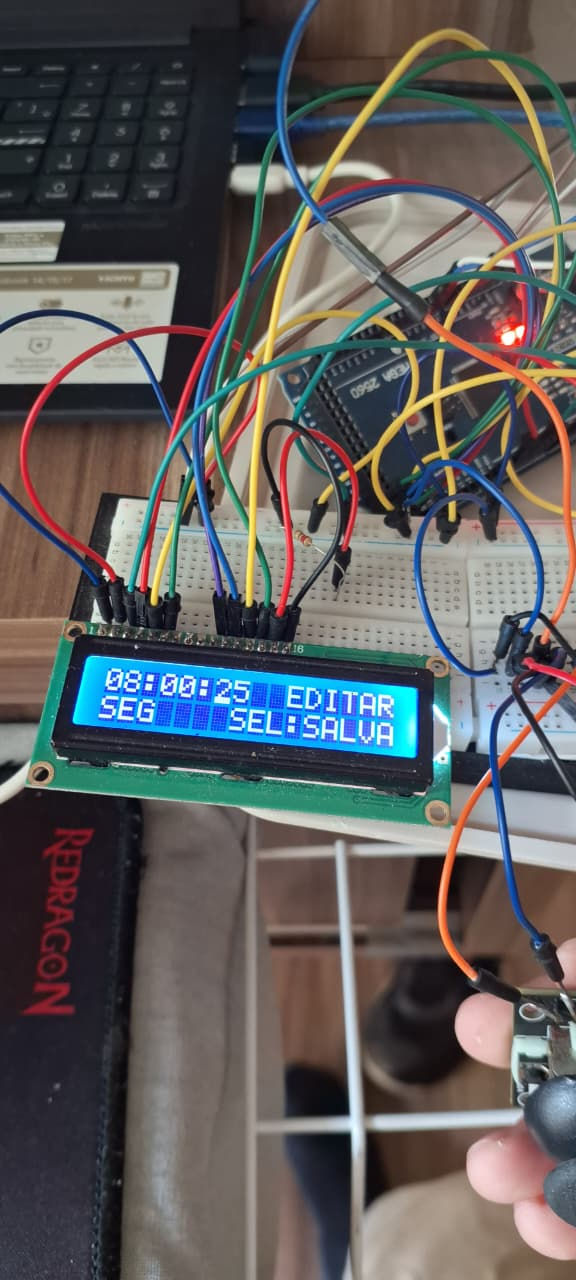
\includegraphics[height=8.1cm]{figuras/04_edicao_segundos.jpg}\hspace{3mm}
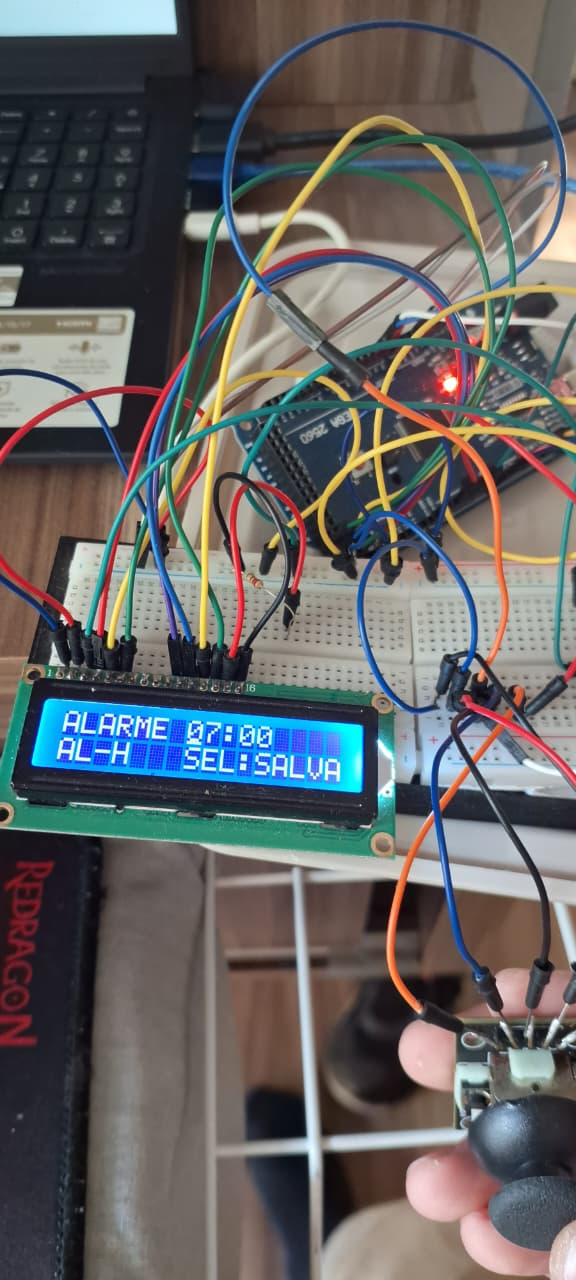
\includegraphics[height=8.1cm]{figuras/08_edicao_alarme.jpg}\hspace{3mm}
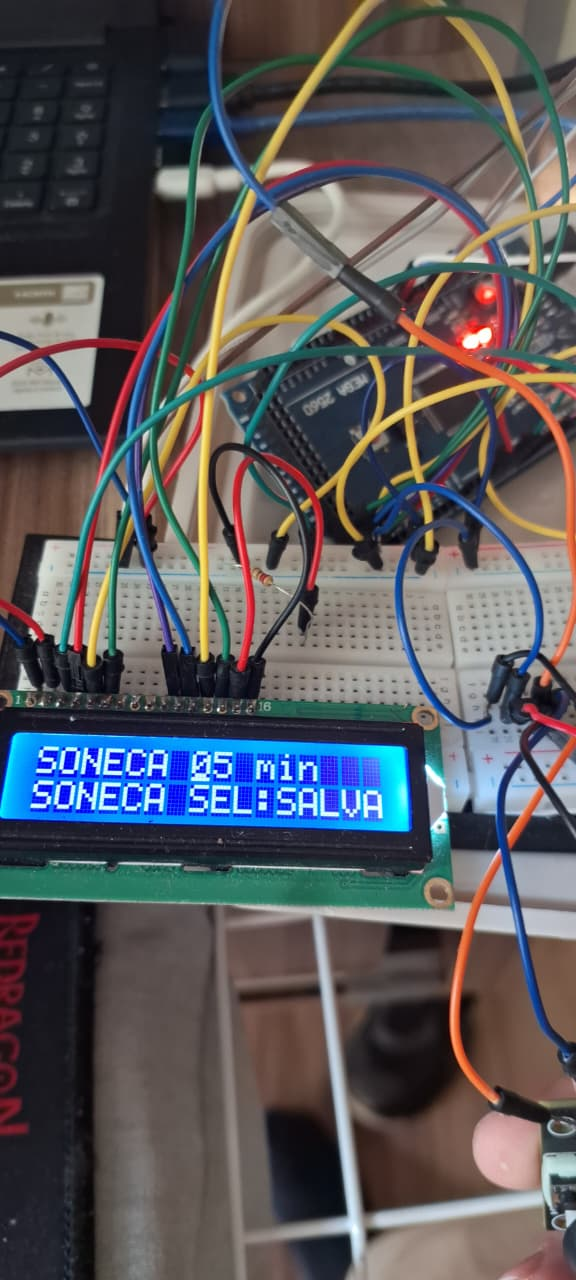
\includegraphics[height=8.1cm]{figuras/09_edicao_soneca.jpg}\hspace{3mm}
\caption{Interface de configuração: edição de segundos, horário do alarme e duração da soneca. Fonte: registro do autor, 08/10/2026.}\label{fig:configuracao}
\end{figure}

A compilação final para Arduino Mega 2560, com Arduino AVR 1.8.8, FreeRTOS 11.1.0-3 e LiquidCrystal 1.0.7, utiliza 18.388 bytes de programa e 729 bytes de dados globais e estáticos. O segundo valor antecede a alocação dinâmica de tarefas e filas; não representa o consumo total de SRAM em execução. O ensaio automatizado do núcleo extraído do próprio sketch aprova 13 grupos de verificações, incluindo calendário, soneca na meia-noite, recuperação de intervalos, edição de segundos, debounce, rollover e limites das linhas do LCD. O teste de seis horas utiliza contagens nominais para verificar a aritmética do calendário.

A solução atende à proposta de alarme com RTOS por meio de quatro tarefas com responsabilidades definidas, interface local e sinalização visual e sonora. O estado com dono único elimina o compartilhamento desnecessário do calendário; a fila expressa a intenção do usuário e a caixa de uma posição transporta o estado atual dos periféricos. O Timer1 separa a evolução do relógio da cadência do escalonador, e o prazo relativo preserva a soneca durante a mudança de dia. O resultado integra máquina de estados, interrupções e serviços do FreeRTOS, demonstrando que organização concorrente e precisão física são aspectos complementares do projeto embarcado.

\FloatBarrier
\printbibliography[heading=bibnumbered,title={Referências}]
\end{document}
